\documentclass[a4paper,10pt]{article}
\usepackage[utf8]{inputenc}
\usepackage[numbers]{natbib}
\bibliographystyle{naturemag}
% amsmath package, useful for mathematical formulas
\usepackage{amsmath}
% amssymb package, useful for mathematical symbols
\usepackage{amssymb}
\usepackage{url}
\usepackage{graphicx}
% Our defs 
\def \rr {$R_{t}\:$}
%opening
\title{Supplementary material to ``Estimating the Attack Ratio of Dengue 
Epidemics under Time-varying 
Force of Infection using Aggregated Notification Data''}
\author{Flavio Code\c{c}o Coelho and Luiz Max de Carvalho}

\begin{document}

\maketitle

\section*{A remark on prior distributions and tail behaviour of the 
distribution of $R_t$}
\label{sec:tails}
There are a number of approaches to deriving the distribution of \rr.
Alternatively to the approach described in the main text~\cite{mantel}, one 
could use the conditional distribution of \rr on 
$Y_{t+1}$ and $Y_t$ as defined in equation A7 of Nishiura et 
al.~\cite{nishiura}:
\begin{equation}
\label{seq:unorm}
f_{R}(R_{t}) = (Y_tR_{t})^{Y_{t+1}} e^{-Y_tR_{t}}
\end{equation}
Noticing the kernel of (\ref{seq:unorm}) is that of a gamma distribution with 
$a_2 = Y_{t+1}+1$ and $b_2 = Y_t$, we obtain a proper density from which to 
construct $c_{\alpha}(R_t)$, simply by computing the appropriate quantiles of 
said distribution.
 This density is
\begin{equation}
\label{seq:densityNishiura}
f_N(R_t| a_2, b_2) =  \frac{b_2^{a_2}}{\Gamma(a_2)} R_t^{a_2-1} e^{-b_2 R_t}
\end{equation}

In order to decide which approach to take, it may be of use analysing the 
tail behaviour of the derived distributions for \rr. 
Consider the case of using a flat $Uniform(0, 1)$ prior for $\theta_t$.
With $a_0 = b_0 = 1$, $a_1 = a_2$ and $b_1 = b_2 + 1$.
The beta prime (inverse beta distribution) will have heavier tails compared to 
the conditional distribution proposed by~\cite{nishiura}, thus providing more 
conservative confidence/credibility intervals.
To see that one needs simply take the ratio of the Beta prime and Gamma 
(unnormalized) densities and evaluate the limit as $R_t$ goes to infinity:
\begin{equation}
 \label{seq:densityratio}
 \lim_{R_t\to\infty}\frac{f_P(R_t| a_1, b_1)}{f_N(R_t| a_2, b_2)} =  
\lim_{R_t\to\infty}\frac{e^{Y_{t}R_t}}{(1 +R_t)^{Y_{t} + Y_{t +1}+2}} = \infty
\end{equation}
Finally, note that we deliberately construct $c_{\alpha}(R_{t})$ as a 
equal-tailed $100\alpha\%$ credible set, rather than a less conservative 
highest posterior density (HPD) interval.

As a side note, the Bayesian approach presented in this 
paper will give similar results to orthodox confidence intervals~\cite{wilson} 
and~\cite{clopper} for $Y_{t+1}$ and $Y_t >> 1$.
Under the flat  uniform prior for $\theta_t$, the Bayesian posterior 
credibility 
interval is nearly indistinguishable from the confidence interval proposed by 
Clopper \& Pearson (1931)~\cite{clopper} for $Y_{t+1}, Y_t > 20$.
Note also that the uniform prior ($Beta(1, 1)$) for $\theta_t$ constitutes a 
poor 
prior 
choice mainly because the induced distribution for \rr is only well-defined for 
$b_0 > 2$.

An advantage of the Bayesian approach is that one can devise prior 
distributions for $\theta_t$ taking advantage of the intuitive parametrization 
and flexibility of the beta family of distributions.
Prior elicitation can also be done for \rr and the hyper-parameters directly 
plugged into the prior for $\theta_t$. 
One can, for example, choose prior mean and variance for \rr and find $a_0$ 
and $b_0$ that satisfy those conditions.
Let $m_0$ and $v_0$ be the prior expectation and variance for $R_t$. 
After some tedious algebra one finds
\begin{align}
\label{seq:elicitation}
a_0 &= \frac{m_0v_0 + m_0^3 + m_0^2}{v_0} \\
b_0 &= \frac{2v_0 + m_0^2 + m_0}{v_0}
\end{align}
If one wants only to specify $m_0$ and the coefficient of variation $c = 
\sqrt{v_0}/ m_0$ for $R_t$ \textit{a priori}, some less boring 
algebra gives:
\begin{align}
\label{seq:elicitationcv}
a_0 &= \frac{m_0^3c^2 + m_0^3 + m_0^2}{m_0^2c^2} \\
b_0 &= \frac{2m_0^2c^2 + m^2 + m}{m_0^2c^2}
\end{align}

This approach thus makes it possible to incorporate epidemiological knowledge 
about disease Biology (e.g. the magnitude of $R_0$) into the computation of \rr.
This may prove particularly important when disease counts are low and/or close 
to the detection threshold.
We provide an R script to perform the above elicitation at 
\url{https://github.com/fccoelho/paperLM1/blob/master/R/elicit_Rt_prior.R}.

\section*{Estimating $S_0$ from simulated data}
In order to make absolutely clear that the inference methodology proposed can 
recover the true parameter values of the underlying simulation model, we have 
devised a simple simulation experiment. Using the SIR model presented in the 
main paper we have simulated the incidence curve of the  2013 epidemic (2012 in 
table 1 of the article), using $S_0 = 0.0621$ and \rr, as estimated from the 
actual incidence data, and $\tau=1$. Figure \ref{fig:sim_data} shows the 
posterior $S$ and $I$ alongside with the simulated incidence data. It is clear 
the inference can recover the correct value for $S_0$ used to   simulate 
incidence. The script to generate the simulated data and run the inference is in 
the paper's Github repository(\verb|fit_simulated_data.py|).

\begin{figure}
 \centering
 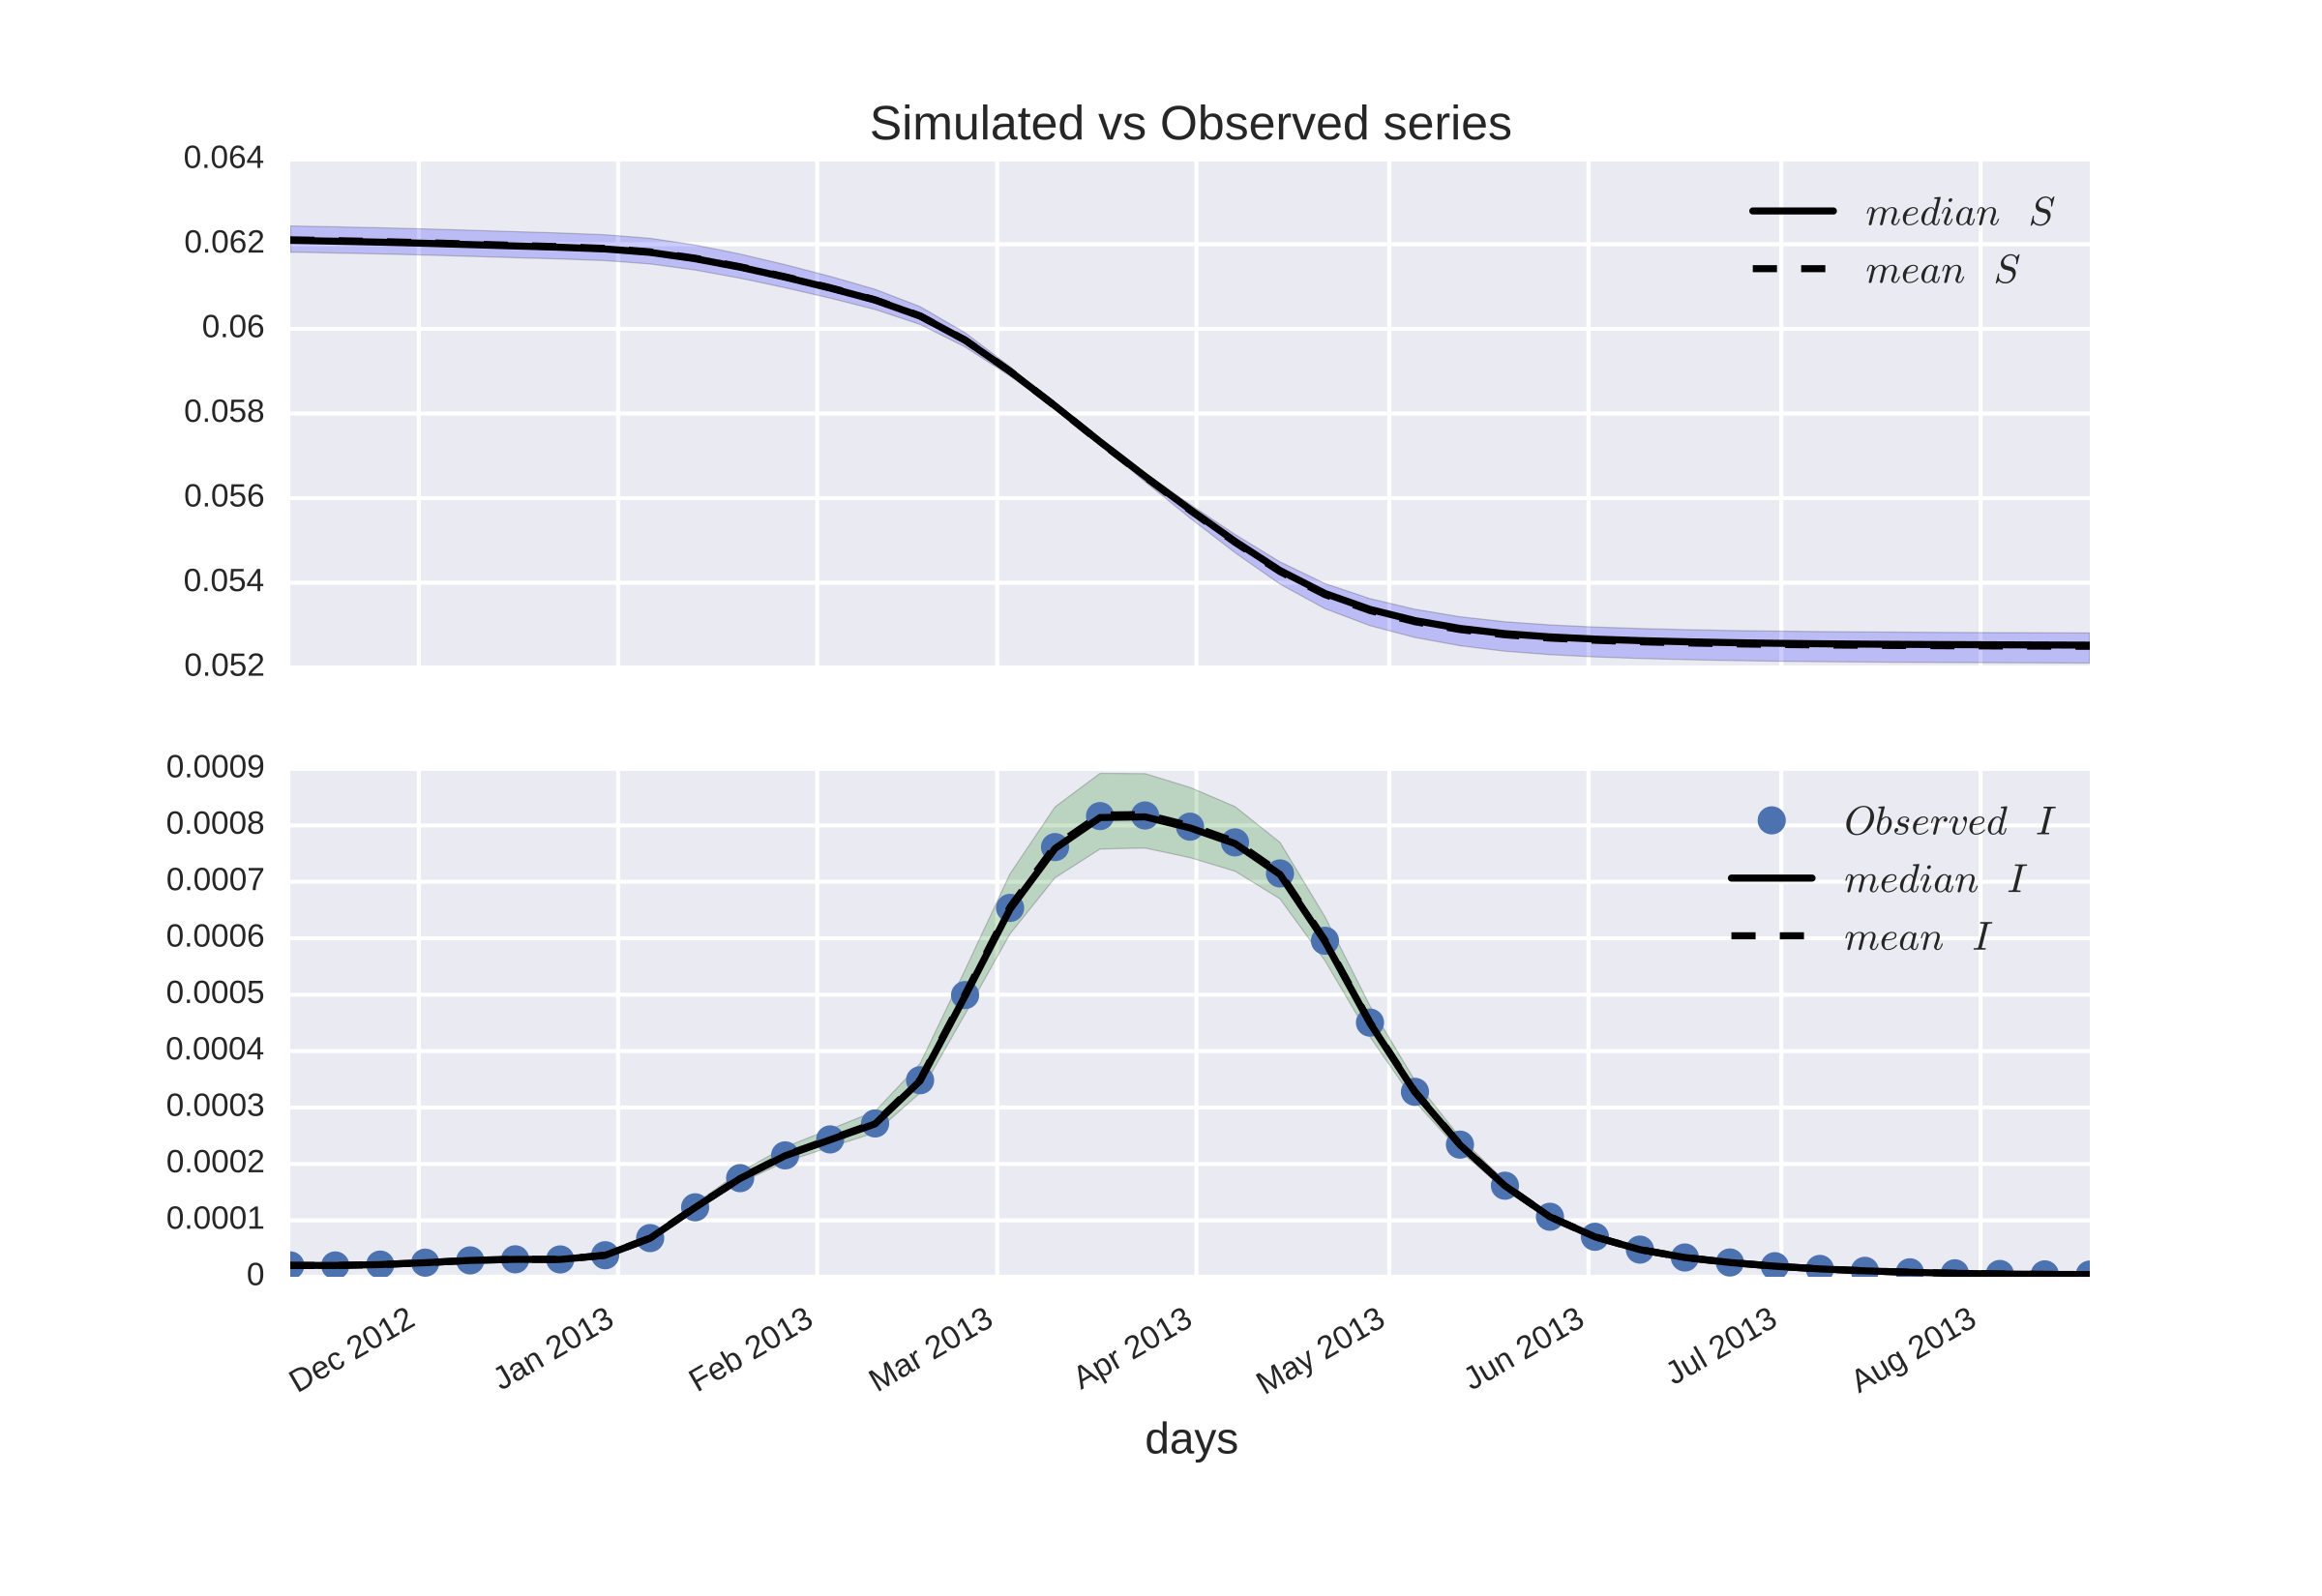
\includegraphics[width=14cm]{./plots/Sim_DengueS2012_11_series.png}
 % Sim_DengueS2012_11_series.png: 0x0 pixel, 300dpi, 0.00x0.00 cm, bb=
 \caption{$S$ and $I$ series fitted to simulated incidence data(blue dots) 
with $S_0=0.0621$, and \rr estimated from real incidence data.}
 \label{fig:sim_data}
\end{figure}

\begin{thebibliography}{1}
\expandafter\ifx\csname url\endcsname\relax
  \def\url#1{\texttt{#1}}\fi
\expandafter\ifx\csname urlprefix\endcsname\relax\def\urlprefix{URL }\fi
\providecommand{\bibinfo}[2]{#2}
\providecommand{\eprint}[2][]{\url{#2}}

\bibitem{mantel}
\bibinfo{author}{Ederer, F.} \& \bibinfo{author}{Mantel, N.}
\newblock \bibinfo{title}{Confidence limits on the ratio of two poisson
  variables}.
\newblock \emph{\bibinfo{journal}{American Journal of Epidemiology}}
  \textbf{\bibinfo{volume}{100}}, \bibinfo{pages}{165--167}
  (\bibinfo{year}{1974}).

\bibitem{nishiura}
\bibinfo{author}{Nishiura, H.}, \bibinfo{author}{Chowell, G.},
  \bibinfo{author}{Heesterbeek, H.} \& \bibinfo{author}{Wallinga, J.}
\newblock \bibinfo{title}{{{T}he ideal reporting interval for an epidemic to
  objectively interpret the epidemiological time course}}.
\newblock \emph{\bibinfo{journal}{J R Soc Interface}}
  \textbf{\bibinfo{volume}{7}}, \bibinfo{pages}{297--307}
  (\bibinfo{year}{2010}).

\bibitem{wilson}
\bibinfo{author}{Wilson, E.~B.}
\newblock \bibinfo{title}{Probable inference, the law of succession, and
  statistical inference}.
\newblock \emph{\bibinfo{journal}{Journal of the American Statistical
  Association}} \textbf{\bibinfo{volume}{22}}, \bibinfo{pages}{209--212}
  (\bibinfo{year}{1927}).

\bibitem{clopper}
\bibinfo{author}{Clopper, C.} \& \bibinfo{author}{Pearson, E.~S.}
\newblock \bibinfo{title}{The use of confidence or fiducial limits illustrated
  in the case of the binomial}.
\newblock \emph{\bibinfo{journal}{Biometrika}} \bibinfo{pages}{404--413}
  (\bibinfo{year}{1934}).

\end{thebibliography}


\end{document}
